\documentclass[tikz,border=5pt]{standalone}

\usepackage{graphicx}
\usepackage{tikz}
\usetikzlibrary{positioning}
\usepackage{comment}

\begin{document}

    \centering
	\definecolor{Mycolor1}{HTML}{1F77B4}
	\definecolor{Mycolor2}{HTML}{FF7F0E}
	\definecolor{Mycolor3}{HTML}{2CA02C}
	\definecolor{Mycolor4}{HTML}{D62728}
	\definecolor{Mycolor5}{HTML}{9467BD}

\definecolor{pltGreen}{rgb}{0.0, 0.5019607843137255, 0.0}
\definecolor{pltRed}{rgb}{1.0, 0.0, 0.0}


%Full Model (Weber)
%
%Bimodal Model (Weber)
%
%original
%
%simulated (1 noise level)
%
%simulated (4 noise levels)
%
%simulated (4 noise levels, bimodal)
%
%lognormal prior: unidentifiable
%
%bimodal prior: identifiable
%
%

\begin{tikzpicture}[
  node distance = 1cm and 1.5cm,
  font=\sffamily,
  every node/.style={inner sep=0, outer sep=0}
]



%%--- Top row: Ground truth
%\node (plot-gt) {};
%\node[right=3.8cm of plot-gt] (plot-gt2) {};
%\node[right=3.8cm of plot-gt2] (plot-gt3) {};
%\node[] at (-0.5,2.4) {\footnotesize{a}}; %Fit to Data}};
%\node[] at (-3.2,1) {\footnotesize{b}}; %Fit to Data}};
%\node[] at (-0.6,1) {\footnotesize{c}}; %Fit to Data}};
%\node[anchor=west] at (-3,2) {
\includegraphics[width=0.65\textwidth]{figures/RunRemington_Free_Zero_VIZ_ForFig8_Human.py_0_0_0.1_200.pdf}};
%\node[anchor=west] at (-3,0.6) {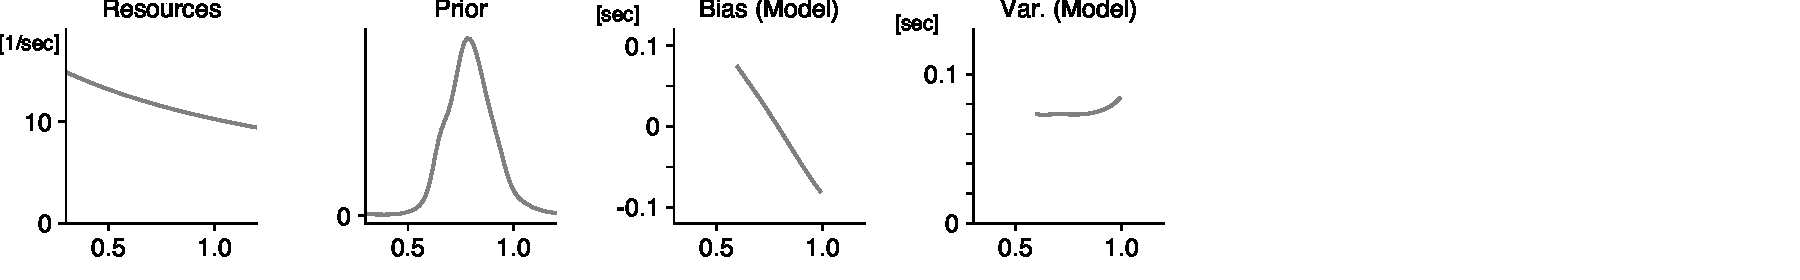
\includegraphics[width=0.65\textwidth]{figures/RunRemington_Free_Zero_VIZ_ForFig8.py_0_0_0.1_200.pdf}};
%%\node[] at (2,0.4) {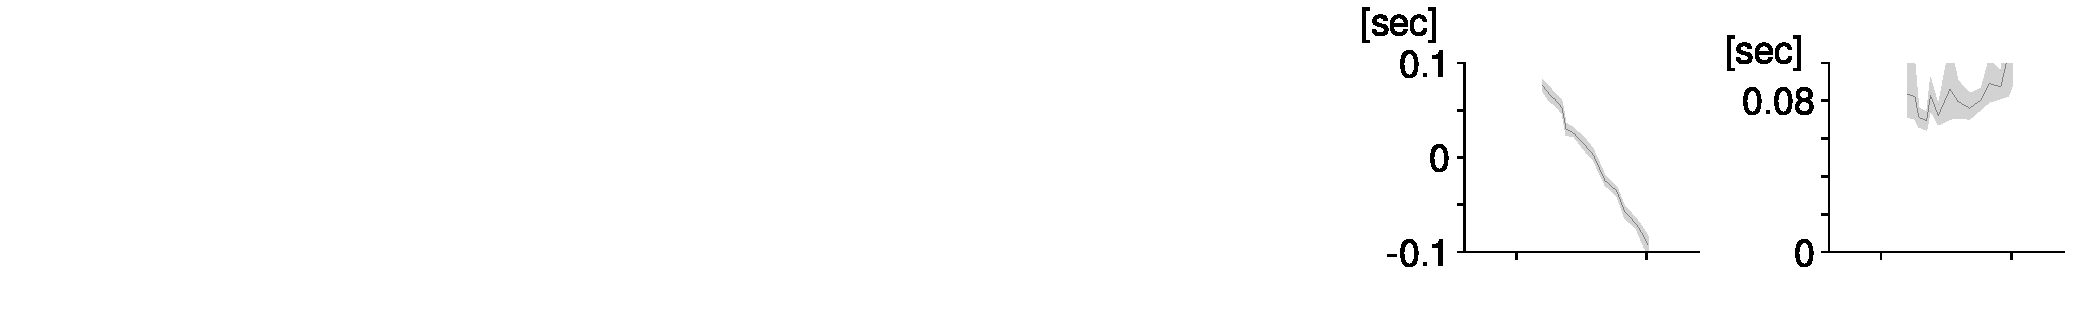
\includegraphics[width=0.45\textwidth]{figures/RunRemington_Lognormal_VIZ_OnlyHuman_MainPaper_ErrBar.py_2_0_0.1_200.pdf}};
%\node[] at (-0.5,-1.9) {\footnotesize{h}}; %Bimodal Prior}};
%\node[] at (-0.5,-0.6) {\footnotesize{f}}; %Bimodal Prior}};
%\node[] at (-3.2,-1.9) {\footnotesize{g}}; %Bimodal Prior}};
%\node[] at (-3.2,-0.6) {\footnotesize{e}}; %Bimodal Prior}};
%
%                                  
%\node[anchor=west] at (-3,-1) {
\includegraphics[width=0.65\textwidth]{figures/RunRemington_Lognormal_VIZ_OnlySimulated_MainPaper_ErrBar.py_0_0_0.1_200_SimulateRemington_Lognormal_OtherNoiseLevels_Zero_DebugFurtherAug.py_200_0_5678_N9000_BIFROMFIT_WEBERFIT.txt.pdf}};
%
%\node[anchor=west] at (-3,-1) {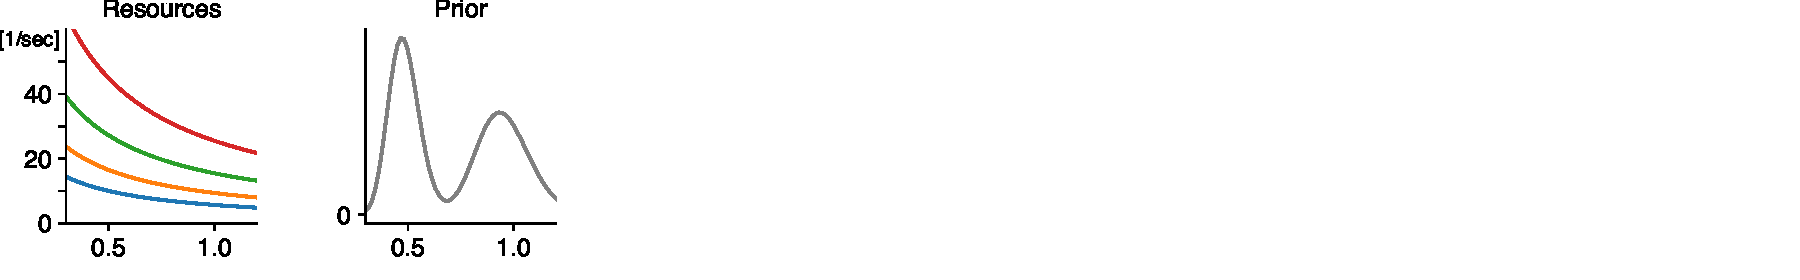
\includegraphics[width=0.65\textwidth]{figures/CounterfactualModel_BasedOnFit_Remington_VIZ_Figure8_OnlyEncPri.py_5678_BIFROMFIT_WEBERFIT_0_0_0.1_200.pdf}};
%
%
%% this would be a full plot of the counterfactual model
%%\node[anchor=west] at (-3,-2.4) {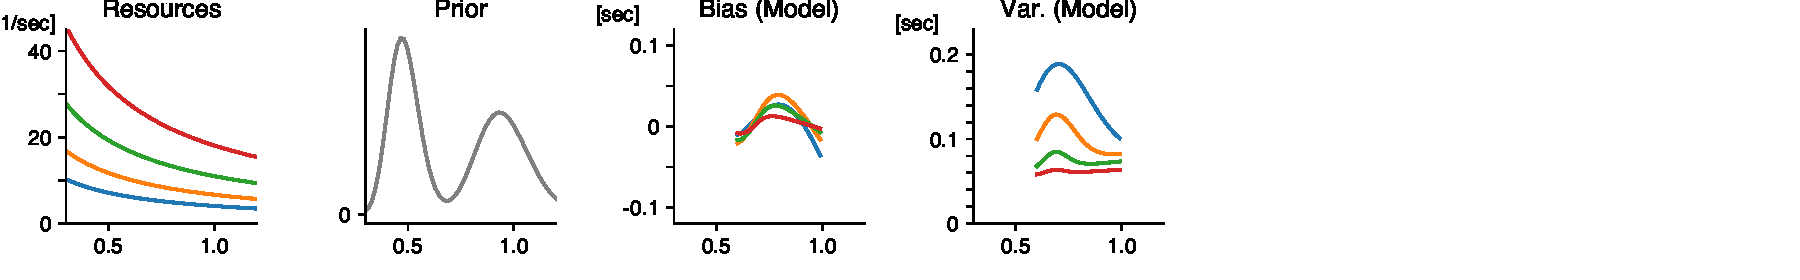
\includegraphics[width=0.65\textwidth]{figures/CounterfactualModel_BasedOnFit_Remington_VIZ_Figure8.py_5678_BIFROMFIT_WEBERFIT_0_0_0.1_200.pdf}};
%
%\node[anchor=west] at (-3,-2.4) {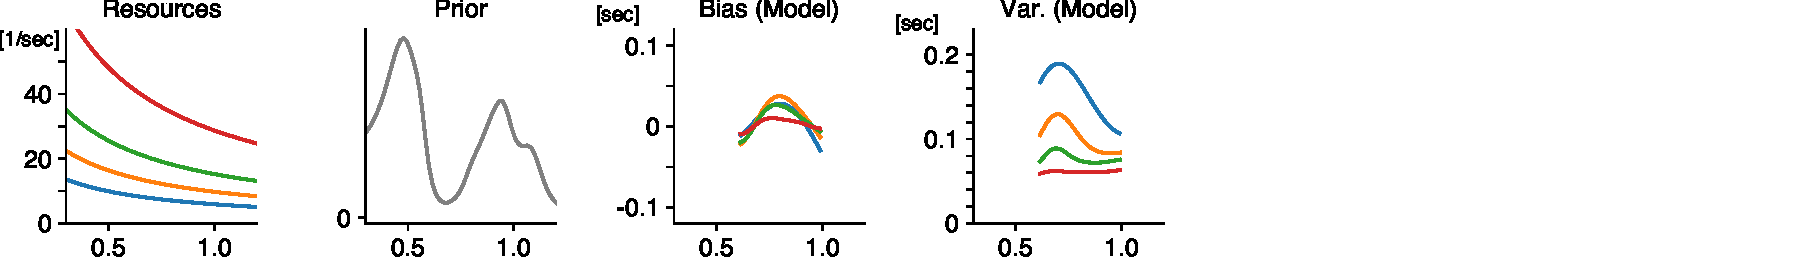
\includegraphics[width=0.65\textwidth]{figures/RunSynthetic_DenseRemington_WeberEncoding_Zero_OnSim_OtherNoiseLevels_VarySize_Round2_VIZ_Figure8.py_SimulateRemington_Lognormal_OtherNoiseLevels_Zero_DebugFurtherAug.py_200_0_5678_N9000_BIFROMFIT_WEBERFIT.txt_0_0_0.1_200.pdf}};
%
%

%\node[] at (2.5,1.8) {\footnotesize{d}}; %Original Data};
%\node[] at (2.5,-0.2) {\footnotesize{i}}; %Simulated};
%\node[] at (4.3,-2) {Simulated (Bimodal)};
\node[] at (0,-0.8) {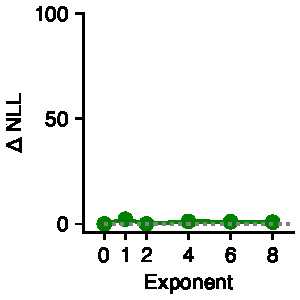
\includegraphics[width=0.15\textwidth]{figures/evaluateCrossValidationResults_Synthetic_Remington_Fig8.py_SimulateRemington_Lognormal_OtherNoiseLevels_Zero_DebugFurtherAug.py_200_0_7_N9000_FROMFIT_WEBERFIT.txt_RelativeLF.pdf}};
\node[] at (0,-0.8) {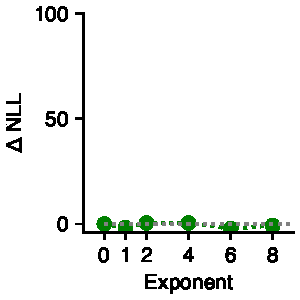
\includegraphics[width=0.15\textwidth]{figures/evaluateCrossValidationResults_Synthetic_Remington_Fig8.py_SimulateRemington_Lognormal_OtherNoiseLevels_Zero_DebugFurtherAug.py_200_0_5678_N9000_FROMFIT_WEBERFIT.txt_RelativeLF.pdf}};
\node[] at (0,-3) {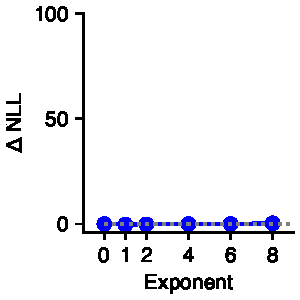
\includegraphics[width=0.15\textwidth]{figures/evaluateCrossValidationResults_Synthetic_Remington_Fig8.py_SimulateRemington_Lognormal_OtherNoiseLevels_Zero_DebugFurtherAug.py_200_0_7_N9000_BIFROMFIT_WEBERFIT.txt_RelativeLF.pdf}};
\node[] at (0,-3) {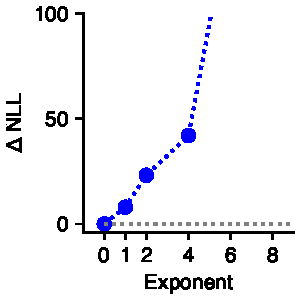
\includegraphics[width=0.15\textwidth]{figures/evaluateCrossValidationResults_Synthetic_Remington_Fig8.py_SimulateRemington_Lognormal_OtherNoiseLevels_Zero_DebugFurtherAug.py_200_0_5678_N9000_BIFROMFIT_WEBERFIT.txt_RelativeLF.pdf}};


\node[] at (-2,-0.8) {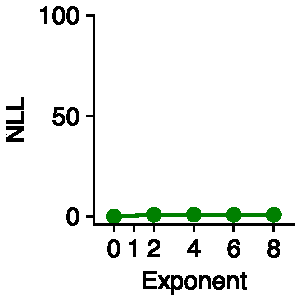
\includegraphics[width=0.15\textwidth]{figures/evaluateCrossValidationResults_Synthetic_Remington_Fig8_WeberEnc.py_SimulateRemington_Lognormal_OtherNoiseLevels_Zero_DebugFurtherAug.py_200_0_7_N9000_FROMFIT_WEBERFIT.txt_RelativeLF.pdf}};
\node[] at (-2,-0.8) {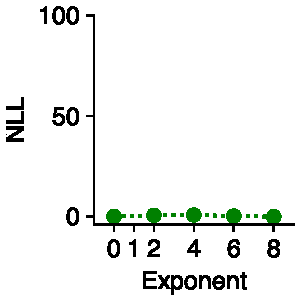
\includegraphics[width=0.15\textwidth]{figures/evaluateCrossValidationResults_Synthetic_Remington_Fig8_WeberEnc.py_SimulateRemington_Lognormal_OtherNoiseLevels_Zero_DebugFurtherAug.py_200_0_5678_N9000_FROMFIT_WEBERFIT.txt_RelativeLF.pdf}};
\node[] at (-2,-3) {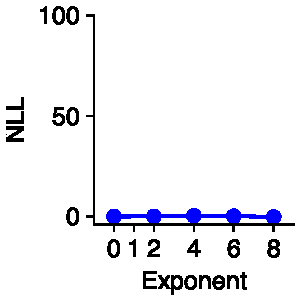
\includegraphics[width=0.15\textwidth]{figures/evaluateCrossValidationResults_Synthetic_Remington_Fig8_WeberEnc.py_SimulateRemington_Lognormal_OtherNoiseLevels_Zero_DebugFurtherAug.py_200_0_7_N9000_BIFROMFIT_WEBERFIT.txt_RelativeLF.pdf}};
\node[] at (-2,-3) {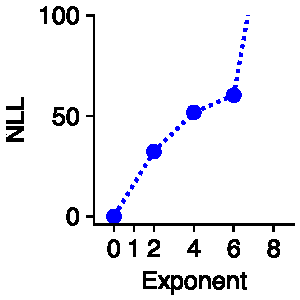
\includegraphics[width=0.15\textwidth]{figures/evaluateCrossValidationResults_Synthetic_Remington_Fig8_WeberEnc.py_SimulateRemington_Lognormal_OtherNoiseLevels_Zero_DebugFurtherAug.py_200_0_5678_N9000_BIFROMFIT_WEBERFIT.txt_RelativeLF.pdf}};

%
%
%\node[font=\tiny\fontfamily{phv}\selectfont, align=center] at (5.2,0.6) {
%  % Matplotlib green: RGB (44, 160, 44) → normalized ≈ (0.1725, 0.6275, 0.1725)
%  \textcolor[rgb]{0.1725,0.6275,0.1725}{----} \\
%  unimodal \\
%  \\
%  \\
%  % Matplotlib blue: RGB (31, 119, 180) → normalized ≈ (0.1216, 0.4667, 0.7059)
%  \textcolor[rgb]{0.1216,0.4667,0.7059}{----} \\
%  bimodal \\
%  \\
%  \\
%  ----- \\
%  1 level \\
%  \\
%  \\
%  - - - \\
%  4 levels
%};
%


\begin{comment}
#for Fitting the models on simulated data with free encoding:
#RunSynthetic_DenseRemington_FreeEncoding_Zero_OnSim_OtherNoiseLevels_VarySize_Round2.py 0 0 0.1 200 SimulateRemington_Lognormal_OtherNoiseLevels_Zero_DebugFurtherAug.py_200_0_5678_N9000_BIFROMFIT_WEBERFIT.txt
#RunSynthetic_DenseRemington_FreeEncoding_Zero_OnSim_OtherNoiseLevels_VarySize_Round2.py 0 0 0.1 200 SimulateRemington_Lognormal_OtherNoiseLevels_Zero_DebugFurtherAug.py_200_0_7_N9000_BIFROMFIT_WEBERFIT.txt
#RunSynthetic_DenseRemington_FreeEncoding_Zero_OnSim_OtherNoiseLevels_VarySize_Round2.py 0 0 0.1 200 SimulateRemington_Lognormal_OtherNoiseLevels_Zero_DebugFurtherAug.py_200_0_5678_N9000_FROMFIT_WEBERFIT.txt
#RunSynthetic_DenseRemington_FreeEncoding_Zero_OnSim_OtherNoiseLevels_VarySize_Round2.py 0 0 0.1 200 SimulateRemington_Lognormal_OtherNoiseLevels_Zero_DebugFurtherAug.py_200_0_7_N9000_FROMFIT_WEBERFIT.txt

#for Fitting the models on simulated data with fixed Weber encoding:
#RunSynthetic_DenseRemington_WeberEncoding_Zero_OnSim_OtherNoiseLevels_VarySize_Round2.py 0 0 0.1 200 SimulateRemington_Lognormal_OtherNoiseLevels_Zero_DebugFurtherAug.py_200_0_5678_N9000_BIFROMFIT_WEBERFIT.txt
#RunSynthetic_DenseRemington_WeberEncoding_Zero_OnSim_OtherNoiseLevels_VarySize_Round2.py 0 0 0.1 200 SimulateRemington_Lognormal_OtherNoiseLevels_Zero_DebugFurtherAug.py_200_0_7_N9000_BIFROMFIT_WEBERFIT.txt
#RunSynthetic_DenseRemington_WeberEncoding_Zero_OnSim_OtherNoiseLevels_VarySize_Round2.py 0 0 0.1 200 SimulateRemington_Lognormal_OtherNoiseLevels_Zero_DebugFurtherAug.py_200_0_5678_N9000_FROMFIT_WEBERFIT.txt
#RunSynthetic_DenseRemington_WeberEncoding_Zero_OnSim_OtherNoiseLevels_VarySize_Round2.py 0 0 0.1 200 SimulateRemington_Lognormal_OtherNoiseLevels_Zero_DebugFurtherAug.py_200_0_7_N9000_FROMFIT_WEBERFIT.txt

# The results are very closely equivalent.
######


python3 RunSynthetic_DenseRemington_WeberEncoding_Zero_OnSim_OtherNoiseLevels_VarySize_Round2_VIZ_Figure8.py 0 0 0.1 200 SimulateRemington_Lognormal_OtherNoiseLevels_Zero_DebugFurtherAug.py_200_0_5678_N9000_BIFROMFIT_WEBERFIT.txt


python3 RunRemington_Free_Zero_VIZ_ForFig8_Human.py 0 0 0.1 200
python3 RunRemington_Free_Zero_VIZ_ForFig8.py 0 0 0.1 200


python3 CounterfactualModel_BasedOnFit_Remington_VIZ_Figure8_OnlyEncPri.py 0 0 0.1 200 9000 BIFROMFIT WEBERFIT 5678   
python3 CounterfactualModel_BasedOnFit_Remington_VIZ_Figure8.py 0 0 0.1 200 9000 BIFROMFIT WEBERFIT 5678   

python3 evaluateCrossValidationResults_Remington_StopNoImpQ_OnlyFree.py

# Can alternatively run these here to instead obtain result with freely fitted encoding
python3 evaluateCrossValidationResults_Synthetic_Remington_Fig8.py SimulateRemington_Lognormal_OtherNoiseLevels_Zero_DebugFurtherAug.py_200_0_5678_N9000_FROMFIT_WEBERFIT.txt green 4 
python3 evaluateCrossValidationResults_Synthetic_Remington_Fig8.py SimulateRemington_Lognormal_OtherNoiseLevels_Zero_DebugFurtherAug.py_200_0_5678_N9000_BIFROMFIT_WEBERFIT.txt blue 4
python3 evaluateCrossValidationResults_Synthetic_Remington_Fig8.py SimulateRemington_Lognormal_OtherNoiseLevels_Zero_DebugFurtherAug.py_200_0_7_N9000_FROMFIT_WEBERFIT.txt green 1
python3 evaluateCrossValidationResults_Synthetic_Remington_Fig8.py SimulateRemington_Lognormal_OtherNoiseLevels_Zero_DebugFurtherAug.py_200_0_7_N9000_BIFROMFIT_WEBERFIT.txt blue 1


python3 evaluateCrossValidationResults_Synthetic_Remington_Fig8_WeberEnc.py SimulateRemington_Lognormal_OtherNoiseLevels_Zero_DebugFurtherAug.py_200_0_5678_N9000_FROMFIT_WEBERFIT.txt green 4 
python3 evaluateCrossValidationResults_Synthetic_Remington_Fig8_WeberEnc.py SimulateRemington_Lognormal_OtherNoiseLevels_Zero_DebugFurtherAug.py_200_0_5678_N9000_BIFROMFIT_WEBERFIT.txt blue 4
python3 evaluateCrossValidationResults_Synthetic_Remington_Fig8_WeberEnc.py SimulateRemington_Lognormal_OtherNoiseLevels_Zero_DebugFurtherAug.py_200_0_7_N9000_FROMFIT_WEBERFIT.txt green 1
python3 evaluateCrossValidationResults_Synthetic_Remington_Fig8_WeberEnc.py SimulateRemington_Lognormal_OtherNoiseLevels_Zero_DebugFurtherAug.py_200_0_7_N9000_BIFROMFIT_WEBERFIT.txt blue 1

python3 RunRemington_Lognormal_VIZ_OnlySimulated_MainPaper_ErrBar.py 0 0 0.1 200 SimulateRemington_Lognormal_OtherNoiseLevels_Zero_DebugFurtherAug.py_200_0_5678_N9000_BIFROMFIT_WEBERFIT.txt


\end{comment}

\end{tikzpicture}
\end{document}
